\documentclass[12pt, a4paper]{article}

\usepackage[utf8]{inputenc}
\usepackage[portuguese]{babel}
\usepackage{amsmath}
\usepackage[T1]{fontenc}
\usepackage{amssymb}
\usepackage{indentfirst}
\usepackage{subfigure}
\usepackage[version=4]{mhchem}
\usepackage[font=small,labelfont=bf]{caption}
\usepackage{multirow}

\usepackage[nottoc]{tocbibind}

\usepackage{geometry}
\geometry{a4paper,
 left=3cm,
 top=3cm,
 bottom=3cm,
 right=3cm
 }

\usepackage{graphicx}
\graphicspath{ {./figures/} }

\title{
{Transições de Fase no Modelo de Ising 2D}\\
{\large Modelação e Física Estatística}
\\ \vspace{3cm}
{
\includegraphics[scale=0.5]{Logo_UA.png}}
\vspace{6cm}
}
\author{Alexandre Rodrigues (92993) \\
	João Inácio	(93039)}
\date{\today}



\begin{document}

	\maketitle
	\newpage
	
	{\small Temos como objetivos principais deste trabalho a implementação de um método Monte-Carlo com fim de estudar a transição de fase num modelo magnético, o modelo de Ising, assim como o seu comportamento crítico. Decidimos implementar o método de Wang-Landau, visto que este estima a densidade de estados conjunta e daí conseguimos tirar todas as variáveis termodinâmicas para quais quer temperaturas ao invés do método de Metropolis. }
	
	{\small Começamos por estudar analítica e numericamente o modelo de Ising numa rede $2 \times 2$, de forma a validar a nossa implementação. Estudamos sistemas maiores, $32 \times 32$, e estimamos os expoentes críticos.}
	
	\section{Modelo de Ising}
	
	O modelo de Ising, nomeado após Ernest Ising que o resolveu no caso de uma dimensão \cite{ising}, considera uma cadeia de partículas de spin-1/2 que só podem interagir com os seus vizinhos mais próximos. Lars Onsager resolveu analiticamente o modelo a duas dimensões \cite{onsager}. Este descobriu que, ao contrário de uma dimensão, há uma transição de fase de um estado ordenado a baixa temperatura para um estado desordenado a alta temperatura. Esta transição ocorre a uma temperatura crítica $T_C$ que a duas dimensões é dada por $T_C \sim 2.269$  \cite{onsager}.
	
	Como neste modelo ocorre uma transição de fase de fase de um estado ordenado para um estado desordenado, este modelo representa as ideias básicas de um material ferromagnético, onde a baixas temperaturas exibe uma magnetização espontânea e a altas temperaturas não exibe magnetização.
	
%	No ano de 1920 Wilhelm Lenz, um físico alemão, deu a Ernest Ising, seu estudante de doutoramento, um exercício em que era considerado uma cadeia uni-dimensional de partículas de spin-1/2 que podiam estar a apontar para cima ou para baixo. Os spins interagiam apenas com os seus vizinhos mais próximos. Cinco anos mais tarde, Ising consegui resolver o modelo, sendo premiado com um doutoramento em física. Este concluiu que a uma dimensão não havia transição de fase e, incorretamente, extrapolou que para dimensões maiores, também não havia transições de fase. Mais tarde, em 1944, um físico americano Lars Onsager resolveu analiticamente o mesmo modelo, mas a duas dimensões. Com isto provou que havia uma transição de fase, de um estado ordenado a baixas temperaturas, onde os spins das partículas alinhavam-se segundo o mesmo eixo, para um estado desordenado a altas temperaturas, onde configurações com spins vizinhos anti paralelos eram favorecidas. Ainda não há uma solução analítica para três u mias dimensões,só conseguimos obter estimativas através de métodos numéricos. Desde então o modelo de Ising é um dos modelos físicos mais publicado e estudo devido à sua simplicidade e transição de fase não trivial.
	
%	Este modelo pode representar um material ferromagnético, onde a baixas temperaturas exibe uma magnetização espontânea e a uma certa temperatura, a temperatura de Curie $T_C$, ocorre uma transição de fase para um estado paramagnético. Metais de transição, Ferro, Níquel, Cobalto, e alguns metais raros, como o Gadolínio, exibem este tipo de comportamento.
	
	O modelo de Ising representa um sistema de partículas de spin-1/2, que podem estar a apontar para cima $(+1)$ ou para baixo $(-1)$, onde só há interação entre partículas vizinhas, o seu Hamiltoniano é escrito 
\begin{equation}
	\mathcal{H} = -\sum_{<i,j>} J_{ij} S_i S_j - H \sum_iS_i,
\end{equation}
onde $J$ é a constante de interação entre spins vizinhos, $S_i$ o valor do spin da partícula no local $i$ e $H$ é um campo magnético externo aplicado. A notação $<i,j>$ do somatório significa que a soma é efetuada sobre os vizinhos da partícula $i$. Se $J>0$, o sistema a temperaturas baixas comporta-se como de uma maneira ferromagnetica e se $J<0$ comporta-se como um sistema anti-ferromagnético.

	Neste trabalho, não vamos estudar o modelo de Ising com um campo magnético aplicado, por isso $H=0$, e vamos considerar que a constante de interação é igual à unidade, $J=1$. Assim o hamiltoniano fica
\begin{equation}
	\mathcal{H} = -\sum_{<i,j>} S_i S_j \equiv -\frac{1}{2} \sum_{ij} S_i S_j.
\end{equation}

	\subsection{Densidade de Estados Conjunta}

	A densidade de estados $g(E)dE$ é definida como o número de microestados disponíveis ao sistema num intervalo de energia de $E$ a $E + dE$. Para um sistema discreto, a densidade de estados $g(E)$ dá-nos o número exato de microestados com energia $E$. Com a densidade de estados conseguimos tirar a função partição canónica, $Z(T)$ e a energia livre de Helmholtz, $F(T)$, em função da temperatura.
	
	Como estamos a avaliar um sistema magnético, é-nos útil saber quantos microestados o sistema tem disponível por energias e magnetizações. Assim, usamos a densidade de estados conjunta, um histograma a duas dimensões que contém informação sobre o número de microestados com uma dada energia $E$ e magnetização $M$, $g(E, M)$. Com a densidade de estados conjunta, conseguimos obter a função partição canónica e a energia livre ambas em função da temperatura e magnetização do sistema.
	
	Para um sistema Ising a duas dimensões numa rede quadrada de lado $L=2$, a densidade de estados conjunta fica
	\begin{table}[h]
	\centering
	\caption{Densidade de estados conjunta para um sistema Ising 2D numa rede quadrada de lado $L=2$. As colunas representam as magnetizações $M$ e as linhas as energias $E$ disponíveis.}
	\label{exact_L2}
	\begin{tabular}{c|ccccc}
	$E \ / \ M$ & $-4$ & $-2$ &  $0$ & $+2$ &  $+4$ \\ \hline
	$-8$  & 1  & 0  & 0 & 0 & 1 \\
	$-4$  & 0  & 0  & 0 & 0 & 0 \\
	$0$   & 0  & 4  & 4 & 4 & 0 \\
	$+4$   & 0  & 0  & 0 & 0 & 0 \\
	$+8$   & 0  & 0  & 2 & 0 & 0
	\end{tabular}
	\end{table}
	

%	Para obter estes  resultados, tivemos de visitar todas os microestados do espaço de fases $(E, M)$, disponíveis ao sistema. Para sistemas pequenos (até $L=4$ numa rede a duas dimensões) isto é fazível, contudo para sistemas maiores, onde o número de configurações fica  muito elevado, este processo fica muito demorado e é ineficiente. Por exemplo uma rede quadrada com lado $L=8$ tem $2^{256} \approx	 1E77$ configurações e já é impossível determinar a densidade de estados através deste método. Na secção 2, iremos apresentar um método eficiente para tal.
	
		\subsection{Relações Termodinâmicas}

	Tendo a densidade de estados conjunta, conseguimos obter quais quer variáveis termodinâmicas num sistema em equilíbrio \cite{stat_mech_book}.  
	A probabilidade de um estado com energia $E_i$, é dada por
\begin{equation}
	P_i = \frac{\sum_q g(E_i, M_q) \exp(-\beta E_i)}{Z},
\end{equation}
onde $\beta$ é definido como $\beta \equiv 1/k_BT$ e $Z$ é a função partição canónica, 
\begin{equation}
	Z = \sum_q Z(T, M_q) = \sum_q \sum_i g(E_i, M_q) \exp(-\beta E_i).
\end{equation}
Com isto conseguimos obter médias de ensemble, 
\begin{equation}
	\langle E \rangle = \frac{1}{Z} \sum_i \sum_q  g(E_i, M_q) E_i \exp(-\beta E_i),
\end{equation}
\begin{equation}
	\langle M \rangle  = \frac{1}{Z} \sum_q \sum_i M_q g(E_i, M_q) \exp(-\beta E_i) \equiv \frac{1}{Z} \sum_q M_q Z(T, M_q).
\end{equation}
$\langle E \rangle$ está relacionado com a capacidade calorifica e $\langle M \rangle$ está relacionado com a suscetibilidade magnética por 
\begin{equation}\label{C_mean}
	\langle C \rangle = \frac{\langle E^2 \rangle - \langle E \rangle^2}{ k_B T^2}, \quad \quad \quad 
	\langle \chi \rangle = \frac{\langle M^2 \rangle - \langle M \rangle^2}{k_B T},
\end{equation}
e usando a segunda lei da termodinâmica conseguimos tirar a entropia.
\begin{equation}\label{S_mean}
	\langle S \rangle= \int \frac{\langle C \rangle}{T} dT.
\end{equation}

	Contudo há uma outra maneira de obter propriedades termodinâmicas, de uma densidade de estados conjunta. Usando a energia livre de Helmholtz, definida por 
\begin{equation}\label{Helm}
	F(T, M) = - k_B ln(Z(T, M)) \equiv U - TS
\end{equation}
e o principio de minimização de energia, conseguimos obter $F_{min} (T) = \min(F(M, T))$, que é definido como a menor energia livre dependente da temperatura que pode ser alcançada pelo sistema.Com isto conseguimos obter $M_{F_{min}}$, $E_{F_{min}}$ e as seguintes variáveis
\begin{equation}\label{C_dev}
	C = - T \frac{\partial^2 F_{min}}{\partial T^2},
\end{equation}

\begin{equation}\label{S_dev}
	S = - \frac{\partial F_{min}}{\partial T}.
\end{equation}

	\subsection{Exemplo: Modelo de Ising numa rede $2 \times 2$}
	
	Na tabela \ref{exact_L2} encontra-se a densidade de estados conjunta para um sistema Ising 2D numa rede quadrada de lado $L=2$. Com isto e com as fórmulas da secção anterior vamos estudar analiticamente o caso mais simples a duas dimensões.  Considerando um sistema de unidades onde $J=1$ e $k_B = 1$ ($\beta \equiv 1/T$), temos

\begin{table}[h]
\centering
	\begin{tabular}{c|c|c|c|c}
	$M$                  & $E$  & $g$ & $Z(T, M)$                          & $F(T, M)$                                   \\ \hline
	4                  & $-8$ & 1       & $\exp(8/T)$                     & $-8$                                        \\ \hline
	2                  & 0  & 4       & 4                                & $-T\ln(4)$                               \\ \hline
	\multirow{2}{*}{0} & 0  & 4       & \multirow{2}{*}{$4+2\exp(-8/T)$} & \multirow{2}{*}{$-T\ln(4+2\exp(-8/T))$} \\  \cline{2-3}
	                   & 8  & 2       &                                  &                                           \\ \hline
	$-2$                 & 0  & 4       & 4                                & $-T\ln(4)$                               \\ \hline
	$-4$                 & $-8$ & 1       & $\exp(8/T)$                     & $-8$                                       
	\end{tabular}
\end{table}

	Para obter as quantidades termodinâmicas desejáveis, temos de calcular a função partição,
	
	\begin{equation}
		Z = \sum_q Z(T, M_q) = 2\exp(8/T) + 2\exp(-8/T) + 12 = 4 \cosh(8 / T) + 12.
	\end{equation}
	
	A energia média é
	\begin{equation}
		\langle E \rangle = - \frac{\partial}{\partial \beta} \ln(Z) = - \frac{\partial}{\partial \beta} \ln(4 \cosh(8 \beta) + 12)
		= -8 \frac{\sinh(8/T)}{\cosh(8/T) + 3}.
	\end{equation}
	
	A magnetização média pode ser calculada pela fórmula apresentada na secção anterior
	\begin{equation}
		\langle M \rangle = \frac{1}{Z} \left( 4\exp(8/T) + 8 -8 -4\exp(8/T) \right) = 0,
	\end{equation}
	o que era de esperar já que o sistema encontra-se em equilíbrio termodinâmico. Por outro lado, a magnetização média absoluta,
	\begin{equation}
		\langle |M| \rangle = \frac{1}{Z} \left( 4\exp(8/T) + 8 +8 +4\exp(8/T) \right) = \frac{4 + 2\exp(8/T)}{\cosh(8/T) + 3}.
	\end{equation}
	
	Podemos ainda calcular a capacidade térmica e a suscetibilidade magnética. 
	\begin{equation}
		\langle  C \rangle = - \frac{1}{T^2} \frac{\partial }{\partial \beta} \langle E \rangle = \frac{1}{T^2} \frac{64}{\cosh(8/T)+3} \left( \cosh(8/T) - \frac{\sinh^2(8/T)}{\cosh(8/T) + 3} \right)
	\end{equation}
	
	\begin{equation}
		\langle  \chi \rangle  = \frac{\langle M^2 \rangle - \langle M \rangle^2}{T}.
	\end{equation}
	A variância da magnetização é dada por
	\begin{equation}
		\langle M^2 \rangle - \langle M \rangle^2 = \frac{32}{Z} \left( \exp(8/T) + 1 \right) - 0^2 = \frac{8(\exp(8/T) + 1)}{\cosh(8/T) + 3}
	\end{equation}
	assim, a suscetibilidade magnética é
	\begin{equation}
		\langle  \chi \rangle = \frac{8(\exp(8/T) + 1)}{T(\cosh(8/T) + 3)}.
	\end{equation}
	
	Estes resultados analíticos podem ser comparados com a solução numérica.
	
	\pagebreak
	
	\section{Método de Wang-Landau}
	
	Em 2001, Fugao Wang e David P. Landau \cite{wl2001, wl2004} propuseram um novo método de Monte-Carlo, chamado método de Wang-Landau (WL). O objetivo deste método é tentar estimar a função de partição canónica 
\begin{equation}
	Z = \sum_E g(E) \exp(-\beta E),
\end{equation}
através da estimação da densidade de estados $g(E)$ via uma random walk, com probabilidade proporcional ao inverso da densidade de estados $\frac{1}{g(E)}$, que produz um histograma plano no espaço de energia. A estimativa de $g(E)$ é melhorada a cada iteração do método.
Este método pode ser usado para estimar a densidade de estados conjunta, realizando uma random walk no espaço de fases $(E, M)$ ao invés do espaço de energias. 

Primeiro começamos num ponto aleatório do espaço de fases, $(E_i, M_i)$,  e com uma estimativa da densidade de estados, normalmente $g(E, M)=1$. Começamos a random walk, efetuando um spin-flip que leva o sistema do estado $(E_i, M_i)$ ao estado $(E_j, M_j)$ e aceitamos esta modificação com uma probabilidade
\begin{equation}
	P((E_i, M_i) \rightarrow (E_j, M_j)) = \min\left(1, \frac{g(E_i, M_i)}{g(E_j, M_j)}\right).
\end{equation}
Quer a nova configuração seja aceite ou rejeitada, estamos no ponto $(E, M)$ do espaço de fases e atualizamos o histograma e a densidade de estados segundo,
\begin{equation*}
	H(E, M) = H(E,M)+1, \quad \quad \quad \quad g(E,M)=f \times g(E,M).
\end{equation*}
Aqui, o parâmetro $f$ e chamado de fator de modificação. Uma escolha razoável para este parâmetro no inicio da simulação é $f_0=e$. Se este é demasiado grande vai induzir erros estatísticos na nossa estimativa, caso seja demasiado pequeno a simulação vai ficar muito demorada. 
Este processo é repetido até obtermos um histograma "plano". Como é impossível obter um histograma $100\%$ plano, definimos um critério para a planicidade do histograma como $\min(H(E, M)) > \langle H(E, M) \rangle \times p$. $p$ é escolhido de acordo com o sistema que estamos a simular. Para sistemas pequenos, $p$ pode ser tão grande como $0.95$, contudo para sistemas maiores a condição de planicidade pode nunca ser satisfeita se $p$ for perto da unidade.

Quando o histograma fica plano, fazemos $H(E, M) = 0$ e reduzimos o fator de modificação $\sqrt{f_{i}} \rightarrow f_{i+1}$, de forma a obter uma melhor estimativa da densidade de estados conjunta a cada iteração da simulação. Repetimos isto até que o valor de $f$ seja menor que um dado $f_{final}$, que normalmente define-se como $f_{final}  \sim 1+1E-8$.

No final da simulação temos que normalizar a densidade de estados. Para tal, podemos usar o facto de 
\begin{equation}
	\sum_{E,M} g(E,M) = 2^N,
\end{equation}
onde $N$ é o número de partículas no sistema.
	
	\pagebreak	
	
	\section{Resultados}
	
	\subsection{Modelo de Ising numa rede $2 \times 2$}	
	
	De forma a verificar que a nossa implementação do método Wang-Landau está correta, decidimos calcular a densidade de estados conjunta de um sistema Ising $2\times 2$ e comparar com a solução calculada analiticamente na secção 1.  Obtivemos os seguintes resultados,
	
	\begin{figure}[h]
		\centering
		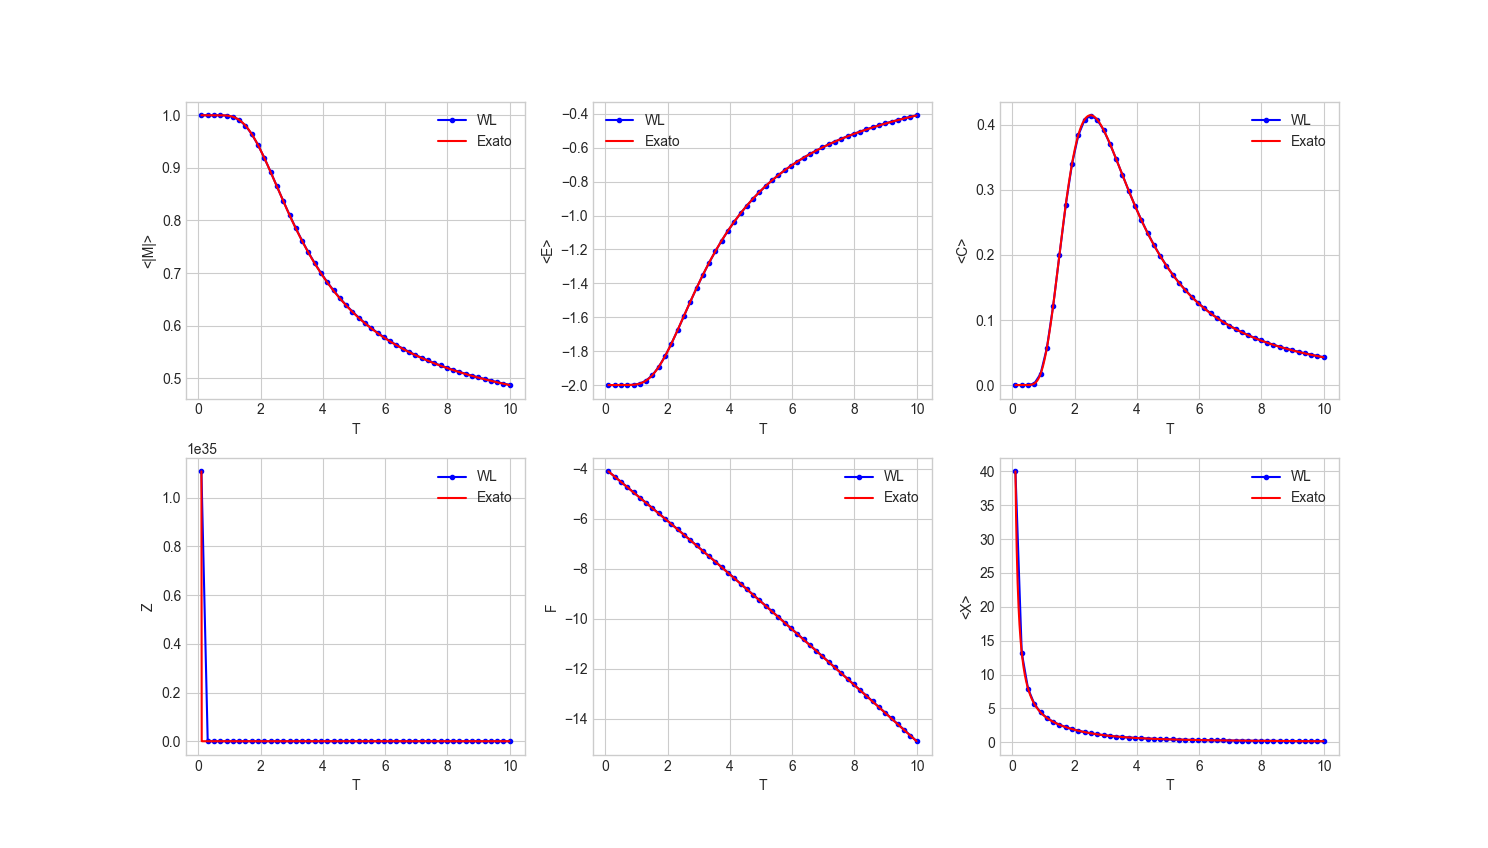
\includegraphics[scale=0.4]{L2.png}
		\caption{Comparação de quantidades termodinâmicas calculadas a partir da densidade de estados estimada pelo método de Wang-Landau versus a solução analítica para um sistema Ising $2 \times 2$.}
		\label{L2}
	\end{figure}
	
	Todas as quantidades termodinâmicas calculadas pelo método estão de acordo com os resultados analíticos, por isso damos a nossa implementação como validada. 
	
	\subsection{Modelo de Ising numa rede $32 \times 32$}
	
	De forma a obter quantidades termodinâmicas pela minimização da energia livre temos de ter um sistema suficientemente grande para que o erro numérico no cálculo das derivadas do mínimo de energia em função da temperatura seja suficientemente pequeno tal que possa ser desprezado. Um sistema 2D $32 \times 32$ já tem $513$ valores de magnetizações possíveis, logo o erro das derivadas não vai ser significante.
	
	Em primeiro lugar temos de obter $F_{min}$, definido como $F_{min} (T) = \min(F(M, T))$. Para tal, calculamos a energia livre de Helmholtz em função da magnetização, pela equação \ref{Helm}. Obtém-se o gráfico da figura \ref{F_L32}.
	\begin{figure}[h]
		\centering
		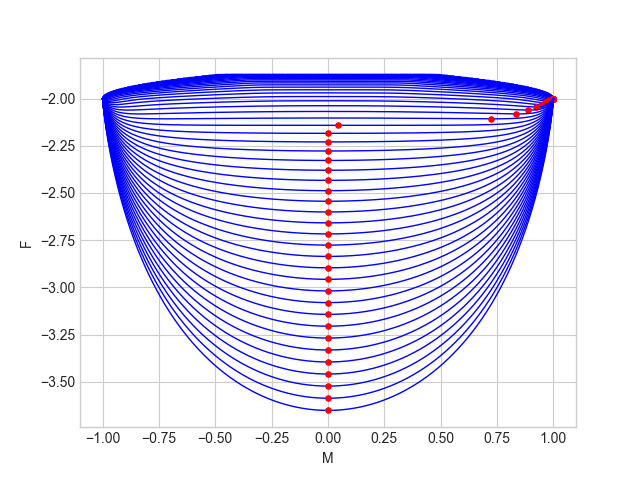
\includegraphics[scale=0.45]{F_L32.png}
		\caption{Energia livre em função da temperatura e magnetização. Cada linha representa um valor de temperatura diferente. Os pontos a vermelho indicam o par $(F, M)$ mínimo para uma dada temperatura.}
		\label{F_L32}
	\end{figure}
Os pontos marcados a vermelho são as magnetizações que minimizam a energia para uma dada temperatura, de acordo com o principio da minimização da energia livre. Com esses pontos conseguimos construir o gráfico da figura \ref{M_L32} de $M_{F_{min}}$ em função da temperatura.

	\begin{figure}[h]
		\centering
		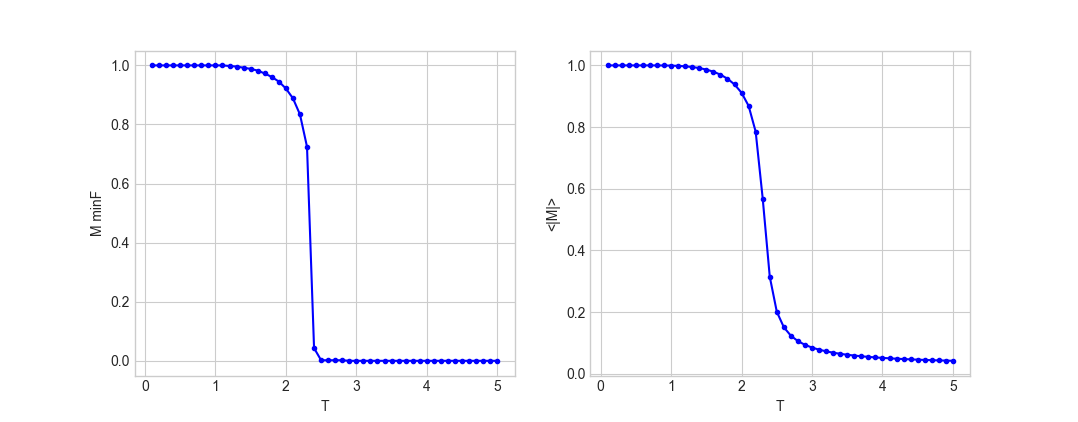
\includegraphics[scale=0.45]{M_L32.png}
		\caption{Magnetização em função da temperatura obtida de duas maneiras. No gráfico da esquerda a magnetização foi obtida pela minimização da energia livre. No gráfico da direita a magnetização é a média de ensemble.}
		\label{M_L32}
	\end{figure}
	Esperaríamos que estes gráficos fossem iguais, já que ambos representam a magnetização do sistema em função da temperatura. Isto é verdade para uma rede de tamanho infinito. Para redes finitas, a forma da curva do gráfico da esquerda é mais parecida à curva da magnetização da rede infinita. Já o gráfico da direita tem uma curva mais achatada, contudo a temperatura onde ocorre a transição de fase aproxima-se mais da temperatura da rede infinita ($T_C(L \rightarrow \infty) \sim 2.269$).
\begin{table}[h]
\centering
\caption{Estimativas de $T_C$ para redes de tamanhos 4, 8, 16 e 32.}
\begin{tabular}{c|c|c}
$L$  & $T_C\ \langle |M| \rangle$ & $T_C\ M_{F_{min}}$ \\ \hline
4  & 2.525                               & 3.395                    \\
8  & 2.423                               & 2.832                    \\
16 & 2.371                               & 2.525                   \\
32 & 2.320                               & 2.371                 
\end{tabular}
\end{table}	

	Tendo a energia livre mínima para uma dada temperatura conseguimos usar as equações \ref{C_dev} e \ref{S_dev} para calcular os valores exatos do calor específico e da entropia. Analisando o gráfico \ref{C_S_L32} conseguimos observar que, outra vez, a forma das curvas obtidas pela minimização da energia livre aproximam a forma da curva na rede infinita, enquanto os valores obtidos pela média do ensemble têm uma temperatura de transição de fase mais próxima da temperatura da rede infinita.
	
	\begin{figure}[h]
		\centering
		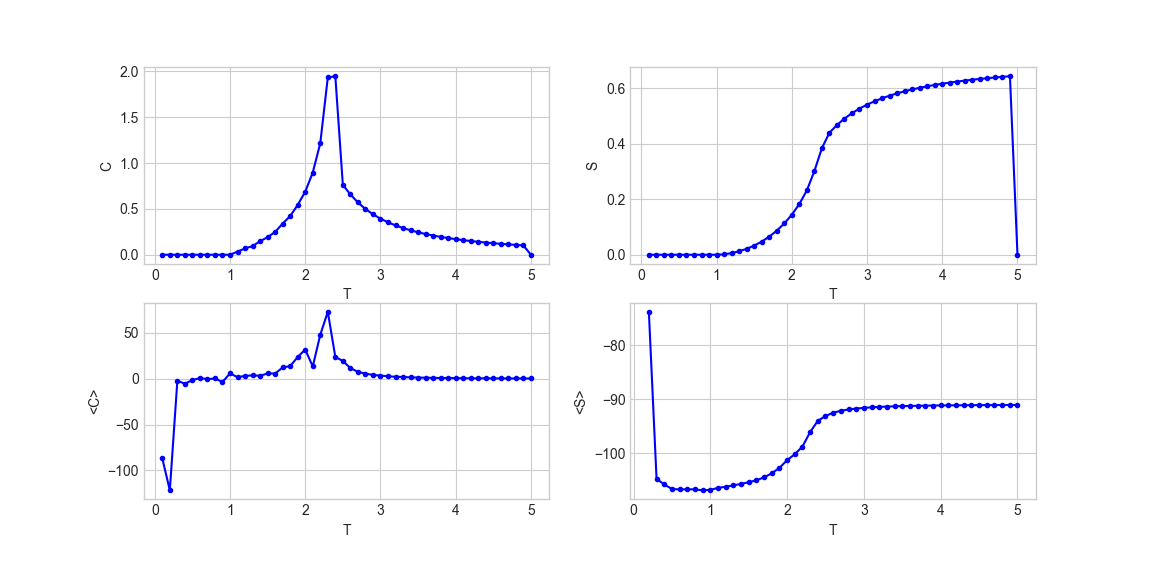
\includegraphics[scale=0.5]{C_S_L32.png}
		\caption{Os dois gráficos de cima são a capacidade térmica e entropia calculadas pelas derivadas de $F_{min}$, os dois gráficos de baixo são as médias da capacidade calorifica e da entropia.}
		\label{C_S_L32}
	\end{figure}
	
	O erro a temperaturas baixas no gráfico da capacidade calorifica média na figura \ref{C_S_L32}, advém do facto do cálculo da densidade de estados conjunta para o sistema $32 \times 32$ não ser o mais preciso. Isto deve-se aos tempos de cálculo serem demasiado elevados e faltou tempo para obter resultados melhores. Como a entropia é calculada pelo integral da capacidade térmica (equação \ref{S_mean}), os seu valores têm um erro mais acrescido.
	
%	\pagebreak
	
	\subsection{Comportamento Crítico}
	
	Num sistema em que ocorre uma transição de fase de segunda ordem, o seu comportamento no limite termodinâmico pode ser descrito por uma energia livre dependente do tamanho \cite{mc_book}, que toma a forma
	\begin{equation}
		F(L, T) = L^{-(2-\alpha)/\nu}\mathcal{F}(t L^{1/\nu}),
	\end{equation}	 
	onde $t$ é a temperatura reduzida $t = \frac{|T_C - T|}{T_C} $. Pela derivação apropriada da energia livre, conseguimos obter varias variáveis termodinâmicas que têm os seus expoentes de escalonamento,
	\begin{align}
		M &= L^{-\beta /\nu} \mathcal{M}^o (t L^{1/\nu}), \\
		\chi &= L^{\gamma /\nu} \mathcal{\chi}^o (t L^{1/\nu}), \\
		C &= L^{\alpha /\nu} \mathcal{C}^o (t L^{1/\nu}),
	\end{align}
	onde $ \mathcal{M}^o (t L^{1/\nu})$, $\mathcal{\chi}^o (t L^{1/\nu})$ e $\mathcal{C}^o (t L^{1/\nu})$ são funções de escalonamento. Os expoentes críticos $\alpha$, $\beta$ e $\gamma$ estão relacionados segundo $2-\alpha=\gamma + \beta$.No ponto exato de transição ($T=T_C$) das propriedades termodinâmicas, as funções de escalonamento reduzem-se a uma constante de proporcionalidade, por isso obtemos
	\begin{align}
		M &\propto L^{-\beta /\nu} \\
		\chi &\propto L^{\gamma /\nu} , \\
		C &\propto L^{\alpha /\nu}.
	\end{align}	
	
	Numa rede finita de tamanho $L$, a transição de fase ocorre a uma temperatura $T_C(L)$. Esta está relacionada com a temperatura crítica do sistema infinito pelo expoente crítico $\nu$. A relação é dada
	\begin{equation}\label{T_C_inf}
		T_C(L) = T_C  + a L^{-1/\nu}.
	\end{equation}
	De acordo com Onsager \cite{onsager}, a temperatura crítica do sistema infinito é $T_C \approx 2.269$, com $\nu=1$. 
		
	O modo mais óbvio para obter os expoentes críticos é fazer uma regressão linear do logaritmo da quantidade pretendida em função do logaritmo do tamanho do sistema. Isto dá-nos uma relação linear em que o declive da reta é o expoente.Neste caso, a ordenada na origem é a constante de proporcionalidade, ou seja, as constantes de escalonamento avaliadas em $T=T_C$. Na determinação dos expoentes críticos assumimos $\nu=1$ para a temperatura crítica ser a temperatura encontrada por Onsager. Assim avaliamos as quantidades termodinâmicas em $T=2.269$.
	
	\begin{table}[h]
	\centering
	\caption{Estimativas dos expoentes críticos do modelo de Ising.}
	\begin{tabular}{c|cc}
	      & Valor Obtido & Valor Teórico \\ \hline
	$\alpha$ & 1.986        & 0             \\
	$\beta$  & 0.122        & 0.125         \\
	$\gamma$ & 1.757        & 1.75         
	\end{tabular}
	\end{table}
	Os valores de $\beta$ e $\gamma$ obtidos são bastante próximos do valor exato, contudo o valor de $\alpha$ está muito longe do valor teórico.Isto deve-se ao facto de haver uma divergência logarítmica na capacidade térmica em $T_C$. Para obter uma boa estimativa do expoente $\alpha$ teríamos que considerar sistemas muito grandes, $L \gg 64$.
	
	Para estimar a temperatura crítica do sistema infinito, temos duas maneiras. Podemos realizar uma regressão linear usando a equação \ref{T_C_inf} ou usar o parâmetro de Binder \cite{mc_book}, definido por
	\begin{equation}
		U_L = 1 - \frac{\langle M^4 \rangle_L}{3\langle M^2 \rangle^2_L}.
	\end{equation}
	Com isto conseguimos traçar uma curva para cada tamanho de sistema considerado. O ponto onde todas estas curvas se encontram é uma estimativa do $T_C$ da rede infinita.
	
	\pagebreak	
	
	\begin{figure}[h]
		\centering
		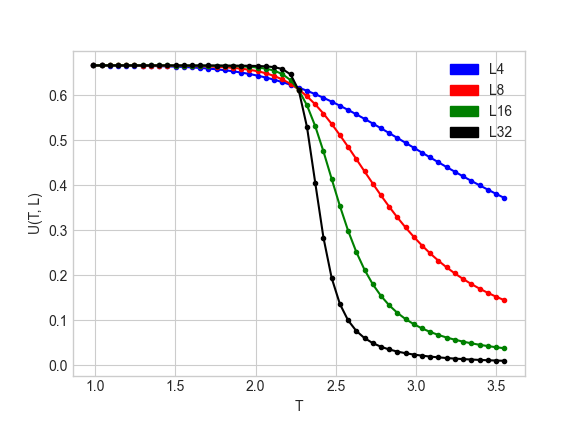
\includegraphics[scale=0.6]{binder_fss.png}
		\caption{Parâmetro de Binder para vários tamanhos de rede, 32, 16, 8 e 4. A abcissa ponto onde todas as curvas se cruzam é uma estimativa da temperatura crítica da rede infinita.}
		\label{binder}
	\end{figure}
	\begin{figure}[h]
		\centering
		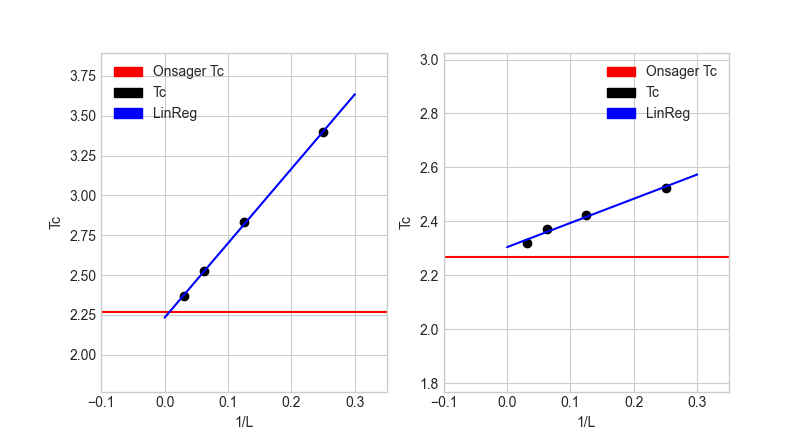
\includegraphics[scale=0.6]{tc_fss.png}
		\caption{Fit de uma regressão linear na equação \ref{T_C_inf}. O gráfico da esquerda tem as temperaturas críticas estimadas pela $M_{F_{min}}$ enquanto no gráfico da direita foram usadas as estimativas de $T_C$ pela $\langle |M| \rangle$}
		\label{ling_reg}
	\end{figure}
	
	O valor da temperatura críticas estimado pelo parâmetro de Binder é aproximadamente $2.233$, enquanto o valor estimado pela regressão linear do $T_C\ M_{F_{min}}$ e $T_C\ \langle |M| \rangle$ é $2.233$ e $2.305$, respetivamente. Para uma estimativa com menor erro, é preferível usar o parâmetro de Binder para estimar o $T_C$ do sistema infinito quando se tem apenas resultados de sistemas pequenos, i.e., $L<32$. Quando se possui resultados de sistemas grandes, quer a estimação através do parâmetro de Binder quer pela regressão linear são precisas.
	
	\pagebreak	
	
	\section{Conclusão}
	
	Conseguimos implementar o método de Wang-Landau com sucesso. Obtivemos resultados que nos permitissem estudar o modelo de Ising a duas dimensões,  com tamanhos de rede 4, 8, 16 e 32. Como não tivemos recursos computacionais suficientes para obter resultados para redes de tamanho maior, alguns dos nossos resultados ficaram imprecisos. Isto é o caso da capacidade térmica calculada pela variância da energia e do expoente crítico $\alpha$, que está correlacionado com a mesma.
	
	De resto, o trabalho correu com sucesso uma vez que conseguimos determinar os expoentes críticos e a temperatura crítica para a rede infinita com alguma exatidão.
		
	\pagebreak
	
	\bibliography{citacoes}	
	\bibliographystyle{ieeetr}
	
\end{document}

